
\documentclass[
                                          %
   12pt,                                % Schriftgroesse 12pt
   a4paper,                             % Layout fuer Din A4
   twoside,                             % Layout fuer beidseitigen Druck
   headinclude,                         % Kopfzeile wird Seiten-Layouts mit beruecksichtigt
   headsepline,                         % horizontale Linie unter Kolumnentitel
   plainheadsepline,                    % horizontale Linie auch beim plain-Style
   BCOR18mm,                            % Korrektur fuer die Bindung
   DIV14,                               % DIV-Wert fuer die Erstellung des Satzspiegels, siehe scrguide
   parskip=half,                        % Absatzabstand statt Absatzeinzug
   bibliography=totoc,                  % Literaturverz. wird ins Inhaltsverzeichnis eingetragen
   captions=tableheading,               % korrekte Abstaende bei TabellenUEBERschriften
%   openany,                            % Kapitel k�nnen auf geraden und ungeraden Seiten beginnen
   listof=totoc,                         % Abbildungs- und Tabellenverzeichnis in Inhaltsverz.
%   pointlessnumbers,                   % Kapitelnummern immer ohne Punkt
%   fleqn,                              % fleqn: Glgen links (statt mittig)
%  draft                               % Keine Bilder in der Anzeige, overfull hboxes werden angezeigt
%   chapterprefix,                      % x. Kapitel �ber Kapitel�berschrift schreiben
     ]{scrbook}[2001/07/30]             % scrbook-Version mind. 2.8j von 2001/07/30

%makeindex Studienarbeit.nlo -s nomencl.ist -o Studienarbeit.nls
\usepackage{ngerman}                    % neue Rechtschreibung
\usepackage[english]{babel}          % falls man in Englisch schreiben will
%\selectlanguage{german}
\selectlanguage{english}               % falls man in Englisch schreiben will
\usepackage{bibgerm}                    % Dt. Bibliothek 

\usepackage[latin1]{inputenc}           % Input-Encodung: latin1 fuer Unix
\usepackage[T1]{fontenc}                % T1-kodierte Schriften, korrekte Trennmuster fuer Worte mit Umlauten
\usepackage{ae}                         % F�r PDF-Erstellung
%\usepackage[hang]{caption2}             % mehrzeilige Captions ausrichten
%\usepackage{pifont}                     % f�r Zahlen im Kreis mit \ding{202} Google: symbols-a4.ps
\usepackage{graphicx}                   % zum Einbinden von Grafiken
\usepackage{float}                      % u.a. genaue Plazierung von Gleitobjekten mit H
\usepackage{tabularx}
\usepackage{amsmath}
\usepackage{amsfonts}
\usepackage{dsfont}
\usepackage{scrhack}
%  \newshadetheorem{definition}{Definition}
%  \newshadetheorem{folgerung}{Folgerung}
%  \newshadetheorem{thm}{Theorem}
  
%\usepackage{draftwatermark}
  
%\DeclareMathOperator{\grad}{grad}

%------------------Anfang Nummerierung Anhang-----------------
 \renewcommand\appendix{\par 
   \setcounter{section}{0}% 
   \setcounter{subsection}{0}% 
   \setcounter{figure}{0}%
   \renewcommand\thesection{\Alph{section}}% 
   \renewcommand\thefigure{\Alph{section}.\arabic{figure}}
   \renewcommand\theequation{\Alph{section}.\arabic{equation}}} 
%------------------Ende Nummerierung Anhang-----------------
%\usepackage{tocbasic}
\usepackage{wrapfig}
\usepackage{longtable}
%\usepackage{subfigure}
\usepackage{subfigure}
%\usepacka{gemes=falsre
%   colorlinks,linkcolor={black},citecolor={black},urlcolor={red},
%   pdfstartview={FitV},unicode,breaklinks=false]{hyperref}
%\usepackage{natbib}
% fuer Stichwortverzeichnis
%\usepackage{makeidx}
%\makeindex
%\renewcommand{\indexname}{Stichwortverzeichnis}
                                        % falls der Index nicht "`Index"' heissen soll
%\addcontentsline{toc}{section}{Stichwortverzeichnis}
                                        % falls das Stichwortverzeichnis im Inhaltsverzeichnis auftauchen soll


%\usepackage[ansinew]{inputenc}
                                        % Input-Encodung: ansinew fuer Windows

%\usepackage[centertags]{amsmath}
                                        % AMS-Mathematik, centertags zentriert Nummer bei split
%\usepackage{latexsym}
                                        % verschiedene Symbole
%\usepackage{textcomp}
                                        % verschiedene Symbole
\usepackage{pstricks}
%\usepackage{pst-all}
%                                        % PostScript Macros
\usepackage{psfrag}
\usepackage{pst-node}
\usepackage{psfrag}

%\usepackage{pstricks-add}  								% Standard PSTricks Paket
%\usepackage{pst-3dplot}								% 3D Plots mit PSTricks 
							% zus�tzliche PSTRicks Funktionalit�t
%\usepackage{rotating}	
%%%%%%%%%%%%%%%%%%%%%%%%%%%%%%%%%%%%%%%%%%%%%%%%%%%%%%
% M A K R O S   U N D   D E F I N I T I O N E N
%%%%%%%%%%%%%%%%%%%%%%%%%%%%%%%%%%%%%%%%%%%%%%%%%%%%%%

%%%%%%%%%%%%%%%%%%%% Symbole %%%%%%%%%%%%%%%%%%%%%%%%%


%%%%%%%%%%%%%%%%%%%%%%% PSTricks %%%%%%%%%%%%%%%%%%%%%%%%%%

%% Zur�cksetzen aller ver�nderten Werte
\newcommand{\psreset}{%
\psset{unit      = 1mm,
       xunit     = 1mm,
       yunit     = 1mm,
       linewidth = 1pt,
       linestyle = solid,
       linecolor = black,
       fillstyle = solid,
       fillcolor = white,
       Beta      = 0,
       Alpha     = 0}}

% Textgr��e
\newcommand{\textscale}{1}
% Liniendicken f�r Zeichnungen
\newlength{\lwFine}   \pssetlength{\lwFine}{0.1mm} % = 0.14mm
\newlength{\lwfine}   \pssetlength{\lwfine}{0.2mm} % = 0.14mm
\newlength{\lwnormal} \pssetlength{\lwnormal}{0.3mm} % = 0.21mm
\newlength{\lwthick}  \pssetlength{\lwthick}{0.5mm}
\newlength{\lwThick}  \pssetlength{\lwThick}{0.75mm} % = 0.64mm%

% verschiedene style Definitionen
\newpsstyle{normal}{arrowsize=1pt 3,arrowlength=2,arrowinset=0, linewidth=\lwnormal}%
\newpsstyle{koordpfeil}{arrowsize=2 0,arrowlength=2.5,arrowinset=0}%
%\newpsstyle{kdpfeil}{arrowsize=1.5 0,arrowlength=1.875,arrowinset=0,linewidth=\lwfine}%
\newpsstyle{masspfeil}{linewidth=\lwfine, arrowsize=2 0,arrowlength=2.5,arrowinset=0}%
%\newpsstyle{dottedline}{linestyle=dotted,dotsep=2pt}

\newpsstyle{PSGraphDash}{plotstyle=line,linewidth=0.8pt,linestyle=dashed,dash=4pt 4pt}
\newpsstyle{PSGraphSolidDot}{plotstyle=line,linewidth=0.8pt,linestyle=solid,showpoints=true}
\newpsstyle{PSGraphDot}{plotstyle=line,linewidth=1.2pt,linestyle=dotted,dotsep=2pt}
\newpsstyle{PSGraphDashDot}{plotstyle=line,linewidth=0.8pt,linestyle=dashed,dash=4pt 2pt 0.6pt 2pt}
\newpsstyle{PSGraphSolid}{plotstyle=line,linewidth=0.8pt,linestyle=solid}
\newpsstyle{PSGraphDashDotDot}{plotstyle=line,linewidth=0.8pt,linestyle=dashed,dash=4pt 2pt 0.6pt 2pt 0.6pt 2pt}
\newpsstyle{PSGraphPoint}{plotstyle=dots,dotstyle=*,dotsize=1.5}
% Schraffuren
\newpsstyle{hatchedu}{fillstyle=hlines,hatchwidth=\lwfine}
\newpsstyle{hatchedd}{fillstyle=vlines,hatchwidth=\lwfine}

%%%%%%%%%%%%%%%%%%%%%%%%% FARBEN %%%%%%%%%%%%%%%%%%%%%%%%%%%%%%%%%

\definecolor{LightBlue}{rgb}{0.68,0.85,0.9}
\definecolor{pink}{rgb}{1.0,0.066,0.9294}
\definecolor{darkgreen}{rgb}{0.251,0.678,0.188}
\definecolor{oker}{rgb}{1.0,0.686,0.3098}
\newgray{lgray}{0.65}
\newgray{llgray}{0.88}

\renewcommand{\rmdefault}{phv} % Arial
\renewcommand{\sfdefault}{phv} % Arial



% Integralzeichen f�r CAUCHY-Hauptwert und finite part nach HADAMARD
\def\Xint#1{\mathchoice
{\XXint\displaystyle\textstyle{#1}}%
{\XXint\textstyle\scriptstyle{#1}}%
{\XXint\scriptstyle\scriptscriptstyle{#1}}%
{\XXint\scriptscriptstyle\scriptscriptstyle{#1}}%
\!\int}
\def\XXint#1#2#3{{\setbox0=\hbox{$#1{#2#3}{\int}$}
\vcenter{\hbox{$#2#3$}}\kern-.5\wd0}}
\def\ddashint{\Xint=}
\def\dashint{\Xint-}
%\usepackage{lscape}
                                        % Seite im Querformat bei Erhalt der Kopfzeile
%\usepackage{verbatim}
                                        % Quellcode einbinden (\verbatiminput)
%\usepackage{multicol}
    \usepackage{colortbl} 
   % \usepackage{hhline}                                   % Mehrspaltiger Text 
%\definecolor{gelb}{rgb}{255,255,0}
%\usepackage{wasysym}
\clubpenalty = 10000                    % Schusterjungen und Hurenkinder vermeiden
                                        % Package f�r Symbole mit \smiley und \frownie 
\widowpenalty = 10000                   % siehe dazu
\displaywidowpenalty = 10000            % http://www.cs.uu.nl/wais/html/na-dir/de-tex-faq/part5.html
  
\usepackage{setspace}                   % Zeilenabstand einstellbar
\onehalfspacing                         % eineinhalbzeilig einstellen
\usepackage{scrpage2}                   % Kopf und Fusszeilen-Layout 
\renewcommand{\headfont}{\normalfont\sffamily}    
                                        % Kolumnentitel serifenlos
\renewcommand{\pnumfont}{\normalfont\sffamily}    
                                        % Seitennummern serifenlos
\pagestyle{scrheadings}
\ihead[]{\headmark}                     % Kolumnentitel immer oben innen
\ohead[\pagemark]{\pagemark}
                                        % Seitennummern immer oben aussen
\ofoot[]{}                              % Seitennummern in der Fusszeile loeschen
%\renewcommand{\captionlabelfont}{\normalfont\sffamily} % Schriftart von Nummerierung der Tabellen und Bildunterschriften

\renewcommand{\chapterpagestyle}{empty} % keine Kopfzeile bei Kapitelanfang
\renewcommand{\titlepagestyle}{empty}   % keine Kopfzeile bei Dokumentanfang
\renewcommand{\indexpagestyle}{empty}   % keine Kopfzeile bei Inhaltsverzeichnis


%\renewcommand{\bibname}{Literatur}
                                        % Literaturverzeichnis wird zu Literatur
%\renewcommand{\figurename}{Bild}
                                        % Abbildung wird zu Bild 
%\renewcommand{\listfigurename}{Abbildungensverzeichnis} 
                                        % Name des Abbildungsverzeichnis

% Schrift mit Serifen auch fuer Ueberschriften benutzen
%\renewcommand*{\sectfont}{\bfseries}
%\renewcommand*{\descfont}{\bfseries}



%%% Literatur und sonstige Referenzen
 \usepackage{cite}                       % Sortierte und zusammengefasste Zitatnummern, nicht mit natbib
% \usepackage[numbers, sort]{natbib}
% \usepackage{natbib}
\usepackage{bookmark}                                        % DIN Literaturverzeichnis; nicht zusammen mit cite verwenden!
\usepackage{varioref}                   % Verbesserte Referenzen
%\usepackage{url}

%\usepackage[intoc]{nomencl}

\typearea[current]{current}             % Neuberechnung des Satzspiegels mit alten Werten nach �nderung von Zeilenabstand,etc


%==================================================
%% PDF-Erzeugung: pdflatex statt latex aufrufen! 
%%\pdfoutput=1                      % PDF-Ausgabe
%\usepackage[pdftex, a4paper,  
 %%   pdftitle={titel},
   % pdfauthor={Nicola Meise},
%    pdfsubject={Studienarbeit},
%    pdfkeywords={wichtige Keywords zur Arbeit},
%5    plainpages=false,pdfpagelabels,
%5    colorlinks  = true,
%5    citecolor   = black,
%    linkcolor   = black,
%    anchorcolor = black,
%    citecolor   = black,
%    filecolor   = black,
%    menucolor   = black,
%    pagecolor   = black,
%    urlcolor    = black,
%    pagebackref = false,
%    ]{hyperref} 

%\usepackage{hyperref}
                                        % externe Links verwenden -> f�r pdftex auskommentieren!!!
%==================================================

\graphicspath{{figs/}{bilder/}}
                                        % Falls texinput nicht gesetzt -> Bildverzeichnisse

%\nomenclature{$d_X$}{Abstandsma� im metrischen Raum $X$}
%\nomenclature{$\textbf{X}$}{TESTTESTTEST}

%\usepackage{blindtext}

%%%%%%%%%%%%%%%%%%%%%%%%%%%%%%%%%%%%%%%%%%%%%%%%%%%%%%%%%%%%%%%
\begin{document}
\pagenumbering{Roman}
\frontmatter
\clearpage
\pagestyle{empty}
\renewcommand*{\chapterpagestyle}{empty}

%% Deckblatt 

\thispagestyle{empty}
~
{\normalsize\fontfamily{phv}\fontsize{14}{14}\selectfont 
\vspace{-3.1cm}
\begin{center}
%\hspace{-7.2 cm}
\begin{minipage}[b]{15cm}
	\begin{center}
	
\includegraphics[width=0.5\textwidth]{uni-logo}
	
	\end{center}
\end{minipage}

\vspace{8mm}
\normalsize \textbf{Universit�t Paderborn\\Fakult�t EIM\\Institut f�r Elektrotechnik und Informationstechnik}

\vspace{8mm}

\includegraphics[width=0.25\textwidth]{Bilder/logo-tet}

\vspace{8mm}
\parbox{\textwidth}{
  \begin{center}
  \LARGE \textbf{TITEL}
  \end{center}
  }


\vspace{1cm}
{ \large \textbf{Diplomarbeit}\\
  \normalsize \textbf{f�r den Diplomstudiengang  Elektrotechnik\\von}\\
  \Large \textbf{NAME}\\
}

\vspace{1cm}
{ \normalsize \textbf{betreut von}\\%[0.9ex]
  \large\textbf{BETREUer}\\
}

\vspace{5mm}
{ \normalsize \textbf{vorgelegt bei}\\%[0.9ex]
  \large \textbf{Prof. Dr.-Ing. Rolf Schuhmann}\\
}

\vspace{1.5cm}
{ \normalsize \textbf{Paderborn, im DATUM}\\%[1.2ex]
}
                 
\end{center}
}
\newpage

                                        % Deckblatt
% Kurzfassung auf Deutsch
%\chapter*{Kurzfassung}
\chapter*{Abstract}
\label{cha:kurzfassung}
Coupling fibers to photonic waveguide leads to normally great energy loss at optical transmissions. This work aims to discuss the coupling interface between tapered and lensed fibers and photonic waveguides and streamline the coupling ability. For this purpose we carried out the analysis by applying numerical simulations with the help of CST MWS and Matlab programs. \\

In this work we have arranged the simulations on following consideration, including relative locations, material composing and waveguide structures. For relative locations we shifted the waveguide in a small range along x, y and z axis respectively. For material composing we have executed simulations in specified surrounding conditions or by changing the waveguide materials.  Simulations for different waveguide structures in this work base on the taper technique and the lens technique. For these simulations we analyzed the coupling efficiency by changing the geometric parameters of both structure.\\

Through the comparison of simulation results we can conclude that changing waveguide material, using tapered or lensed waveguide structures are optimal options. For a realizable implementation we should also consider fabrications and cost of above options.

                                        % Kurzfassung der Arbeit
%\chapter*{Abstract}
\label{cha:abtract} 

This abstract is the translation of the previous \emph{Kurzfassung}, which helps Non-German people to understand your work.


                                        % Abstract der Arbeit
%% Danksagung
\chapter*{Danksagung}
\label{cha:Danksagung} 

%Falls man m�chte kann man hier danken und huldigen.
(optional)

%\nomenclature{$d_X$}{Abstandsma� im metrischen Raum $X$}
% ...
% usw.


%Inhaltsverzeichnis
\cleardoubleemptypage                   % Das Inhaltsverzeichnis auf einer rechten Seite beginnen
\begin{spacing}{1.0}                    % Verzeichnisse werden mit einzeiligem Abstand gesetzt
 \tableofcontents                       % Inhaltsverzeichnis
\end{spacing}

\cleardoubleemptypage
\clearpage
\pagestyle{scrheadings}
% \renewcommand*{\chapterpagestyle}{plain}


%Hauptkapitel
\mainmatter                             % den Hauptteil beginnen

%\include{mainmatter/Einleitung} 	% Einleitung
%Introduction
%\chapter{Introduction}

%introduce
For the research of photonic waveguides it is normally in use to project lights from optical fibers to photonic waveguides (Fiber-to-Chip). In this case the source fiber is generally connected with the laser source because a laser is diffraction limited and highly concentrated. As the signal source optical fibers have usually a larger end face than that of waveguides and the direct coupling from fibers to waveguides cause a very low coupling efficiency. In order to handle this problem tapered lensed fibers (TLF), which are optical fibers with a lens on the end face, are used to replace normal fibers. In Fiber-to-Chip  this new end face of fibers will focus rays emitted from fibers, so that more light power can be coupled into waveguides. The purpose of this work is to analyze the coupling ability from TLF to photonic waveguide through simulations in CST MWS  (CST Microwave Studio\textregistered) and optimize the Fiber-to-Chip interface to achieve more effective coupling.\\

In this work the related basic knowledge for research and analysis will be firstly introduced to make some terms in this work clear for readers. Then the chapter \ref{chp:model} will address readers information about the technical detail of the experimental objects and the modeling procedure. After then we will simulate the unoptimized coupling arrangement and analyze the coupling behavior. In chapter \ref{chp:optim} we will divide the development about the effective coupling between TLF and the waveguide  into four parts. In the first part, we aim at the effect of displacing the waveguide on the coupling efficiency. In the second part we will simulate the unoptimized coupling configuration in oil environment. Then in the third and forth parts we will provide two important techniques of waveguide interface, tapered and lensed interface, for promoting the coupling ability respectively.\\  
                                       
%fundamental
\chapter{fundamental Theories}

\section{Geometric Optics}



%optics
Optical fibers are widely used as a medium for telecommuniction and networking because of varity of advantages.It is flexible,especially permits transmission over longer distances and at higher bandwidths (data rates) than other forms of communication. The Fig.\ref{fig:opticfiber} presents a simplest optical fiber and how lights progate in the fiber. 

\begin{figure}[httbp]
\centering
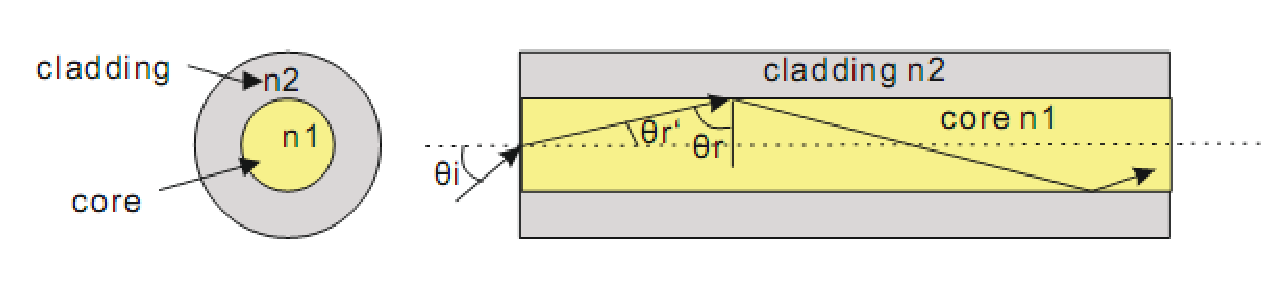
\includegraphics[width=0.8\textwidth]{bilder/opticfiber}
\caption{linght refraction in optic fibers}
\label{fig:opticfiber}
\end{figure}

Optical fiber typically consists of a transparent core with index $n1$ surrounded by a transparent cladding material with a lower index of refraction $n2$. The Light is kept in the core by total internal reflection. This causes the fiber to act as a waveguide.
The principle of the total reflection is explained in \cite{script_FT_TET} with Snell's law. In Fig.\ref{fig:totalreflection} linghts strike a boundary between two different isotropic media with respective refractive indices $n_{1}$ and $n_{2}$ ($n_{1}>n_{2}$), it behaves after Snell's law, which is presented in following mathematical fomular (\ref{eq:snell}).
\begin{figure}[httbp]
\centering
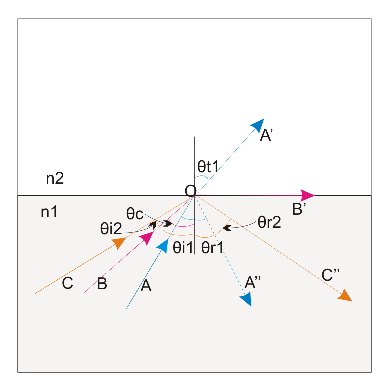
\includegraphics[width=0.6\textwidth]{bilder/totalreflection}
\caption{total reflection}
\label{fig:totalreflection}
\end{figure}

\begin{equation}
n_{1}sin\theta_{i}=n_{2}sin\theta_{t}
\label{eq:snell}
\end{equation}

$\theta_{t}$ is transmission angle or refraction angle.
At a small incidence angle $\theta_{i1}$ a light beam can pass through the boundary and bend to a new course at transmission angle $\theta_{t1}$ in the second meadium.
When the incidence angle is larger than a particular critical angle (\ref{eq:critical_angle}) with respect to the normal to the surface, no light can pass through and all of the light is reflected like (O-C''). In this case the value of $sin\theta_{t}$ in (\ref{eq:sin_transmission_angle}) become larger than one and he mathematical formular of the new transmission angle can be presented by a complex symble $\underline{\theta_{t}}$(\ref{eq:complex_transmission_angle}). $\underline{\theta_{t}}$ is not a real physical angle.

\begin{equation}
\theta_{c}=arcsin(\frac{n_{2}}{n_{1}})
\label{eq:critical_angle}
\end{equation}

\begin{equation}
sin\theta_{t}=\frac{n_{1}}{n_{2}}sin\theta_{i}
\label{eq:sin_transmission_angle}
\end{equation}

\begin{equation}
\underline{\theta_{t}}=\frac{\pi}{2}+j\gamma
\label{eq:complex_transmission_angle}
\end{equation}
with
\begin{equation}
sin\underline{\theta_{t}}=cosh\gamma=\frac{n{1}}{n_{2}}sin\theta_{i},\hspace{2cm}\hfill cos\underline{\theta_{t}}=jsinh\gamma=j\sqrt{cosh^2\gamma-1}
\label{eq:trangle_transmission_angle}
\end{equation}


%Numerical Apertur
Back to the Fig.\ref{fig:opticfiber} the incidence beam originate from the aire into the fiber. There is a maximus coupling angle,so that the beam can be guided under the total reflecting conditions. Its sinus value(\ref{eq:NA}) is called \textbf{Numerical Apertur(NA)}, which indicate the acceptable range of ray beams.

\begin{align}
sin\theta_{i}&=\frac{n_{1}}{n_{0}}sin(90^{o}-\theta_{c})=n_{1}cos\theta_{c} \nonumber\\
&=n_{1}\sqrt{1-sin^{2}\theta_{c}}=n_{1}\sqrt{1-\left(\frac{n_{2}}{n_{1}}\right)^2}=\sqrt{n^2_{1}-n^2_{2}}
\label{eq:NA}
\end{align}


\newpage
\section{Gaussian Beam}

In nature world there is no source of parallel ray. Each beams of lights can be in some ways considered from a simple origin: point light source,which emits light in all directions. Thus a normal light source can not provide a perfect focused beams for optical applications. Laser light (laser radiation)has some very special properties, which very much distinguish it from light with other origins:

\begin{itemize}
\item Laser light is usually delivered in the form of a laser beam, i.e. it propagates dominantly in a well-defined direction with moderate beam divergence. Such a laser beam has a high (sometimes extremely high) degree of spatial coherence. This means that the electric fields at different locations across a beam profile oscillate with a rigid phase relationship. Exactly this coherence is the reason why a laser beam can propagate over long distances without spreading very much in the transverse directions, and why it can be focused to very small spots (high focusability of laser beams).

\item In many but not all cases, laser light also has a high degree of temporal coherence, which is equivalent to a long coherence length. This means that a rigid phase relationship is also maintained over relatively long time intervals, corresponding to large propagation distances (often many kilometers) or to huge numbers of oscillation cycles.
\item The large temporal coherence, quantified with a large coherence time or coherence length, is associated with a narrow spectral bandwidth (or linewidth). (We exclude here the sophisticated case of trains of ultrashort pulses, which can have a large optical bandwidth but nevertheless a high degree of coherence; see the article on coherence for details.) For a visible laser beam, this means that it has a certain pure color, e.g. red, green or blue, but not white or magenta. Some lasers allow a degree of wavelength tuning (e.g. dye lasers). The large coherence length introduces a tendency for the phenomenon of laser speckle, i.e. a characteristic granular pattern which can be observed e.g. when the laser beam hits a metallic surface.

\item In most cases, laser light is linearly polarized. This means that the electric field oscillates in a particular spatial direction (? polarization of laser emission).
\end{itemize}

Optical engineers and researchers working on optics 


 %light beams where the electric field profile in a plane perpendicular to the beam axis can be described with a Gaussian function, possibly with an added parabolic phase profile
To undersstand the behavior of laser beams in optics system some characteristics are in following  introduced. 

In optics and particularly in laser physics, laser beams often occur in the form of Gaussian beams, which are named after the mathematician and physicist Johann Carl Friedrich Gau�. Here, the transverse profile of the optical intensity of the beam with a power $P$ can be described with a Gaussian function:

\begin{align}
I(r,z)&=\frac{P}{\pi w(z)^2 /2}exp(-2\frac{r^2}{w(z)^2})
\end{align}


where the beam radius w(z) is the distance from the beam axis where the intensity drops to $1/e2 (\sim13.5\%)$ of the maximum value. A hard aperture with radius w can transmit $\sim86.5\%$ of the optical power. For an aperture radius of $1.5 w$ or $2 w$, this fraction is increased to $98.9\%$ and $99.97\%$, respectively.

In addition to the Gaussian shape of the intensity profile, a Gaussian beam has a transverse phase profile which can be described with a polynomial of at most second order. A linear phase variation in one direction (not considered further here) describes a tilt, and a quadratic phase variation is associated with divergence or convergence of the beam.


Gaussian beams are usually considered in situations where the beam divergence is relatively small, so that the so-called paraxial approximation can be applied. This approximation allows the omission of the term with the second-order derivative in the propagation equation (as derived from Maxwell's equations), so that a first-order differential equation results. Within this approximation, a Gaussian beam propagating in free space remains Gaussian, except that of course its parameters evolve. For a monochromatic beam, propagating in the $z$ direction with the wavelength $\lambda$, the complex electric field amplitude (phasor) is
\begin{align}
E(r,z) =E_{0}\frac{w_{0}}{w(z)}exp(-2\frac{r^2}{w(z)^2})exp(-i[kz-arctan\frac{z}{z_{R}}+\frac{kr^2}{2R(z)}])
\end{align}

with the peak amplitude $|E0|$ and beam radius w0 at the beam waist, the wavenumber $k = 2\pi /\lambda$, the Rayleigh length $z_{R}$ (see below) and the radius of curvature $R(z)$ of the wavefronts. The oscillating real electric field is obtained by multiplying the phasor with $exp(i 2\pi ct/ \lambda)$ and taking the real part.

\begin{figure}
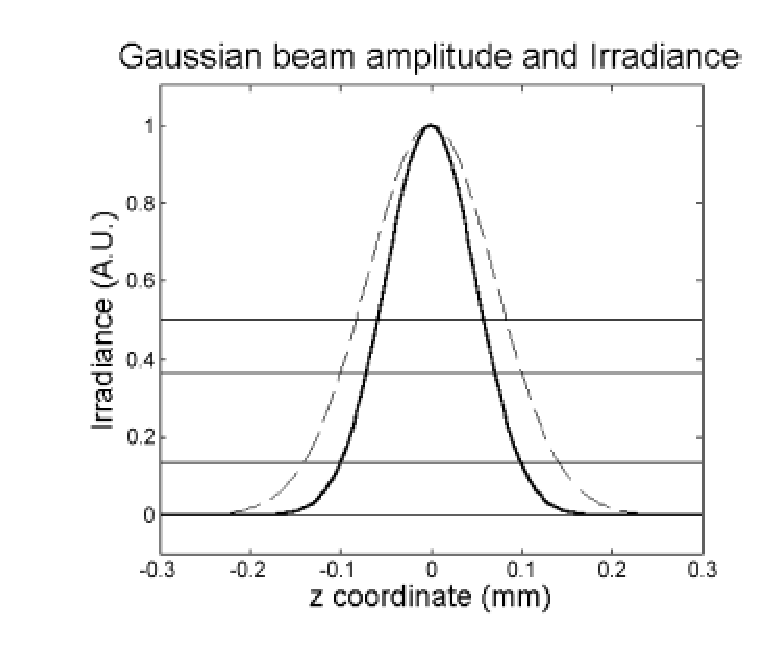
\includegraphics[width=0.8\textwidth]{bilder/gussian_verteilung}
\caption{Transversal profie of the Gussian beam amplitude at the beam waist (dashed line) and irradiance (solid line). Both of them have been normalized to the maximum value. The value of the width of the beam waist $\omega_{0}$ is 0.1 mm. The horizontal lines represent  (in increasing value)the $1/e^{2}$ of the maximum irradiance, the $1/e$ of the maximum amplitude, and the 0.5 of the maximum irrance and amplitude.}
\label{discretization_material}
\end{figure}


\newpage
\section{Finite Integration Method}
%FIT

%\begin{align}
%%\[
%\oint_{\partial A}\vec{E}\cdot\mathrm{d}\vec{s}=
%-\frac{\mathrm{d}}{\mathrm{d}t}\int_{A}\vec{B}\cdot\mathrm{d}\vec{A}\\
%%\]
%%\\
%%\[
%\oint_{\partial A}\vec{H}\cdot\mathrm{d}\vec{s}=
%\int_{A}(\frac{\partial\vec{D}}{\partial t}+\vec{J})\cdot\mathrm{d}\vec{A}\\
%%\]
%%\\
%%\[
%\oint_{\partial V}\vec{D}\cdot\mathrm{d}\vec{A}=
%\int_{V}\rho\mathrm{d}V\\
%%\]
%%\\
%%\[
%\oint_{\partial V}\vec{B}\cdot\mathrm{d}\vec{A}=0
%%\]
%\end{align}
The Finite Integration Theory(FIT) is a numerical simulation method,which was introduced at 1976 by Thomas Weiland to solving the electromagnetical problems after the Maxwell's functions.

\begin{align}
\oint_{\partial A}\vec{E}\cdot\mathrm{d}\vec{s}&=
-\frac{\mathrm{d}}{\mathrm{d}t}\int_{A}\vec{B}\cdot\mathrm{d}\vec{A}\\
\oint_{\partial A}\vec{H}\cdot\mathrm{d}\vec{s}&=
\int_{A}(\frac{\partial\vec{D}}{\partial t}+\vec{J})\cdot\mathrm{d}\vec{A}\\
\oint_{\partial V}\vec{D}\cdot\mathrm{d}\vec{A}&=
\int_{V}\rho\mathrm{d}V\\
\oint_{\partial V}\vec{B}\cdot\mathrm{d}\vec{A}&=0
\end{align}



%fig: discretization of the material
\begin{figure}
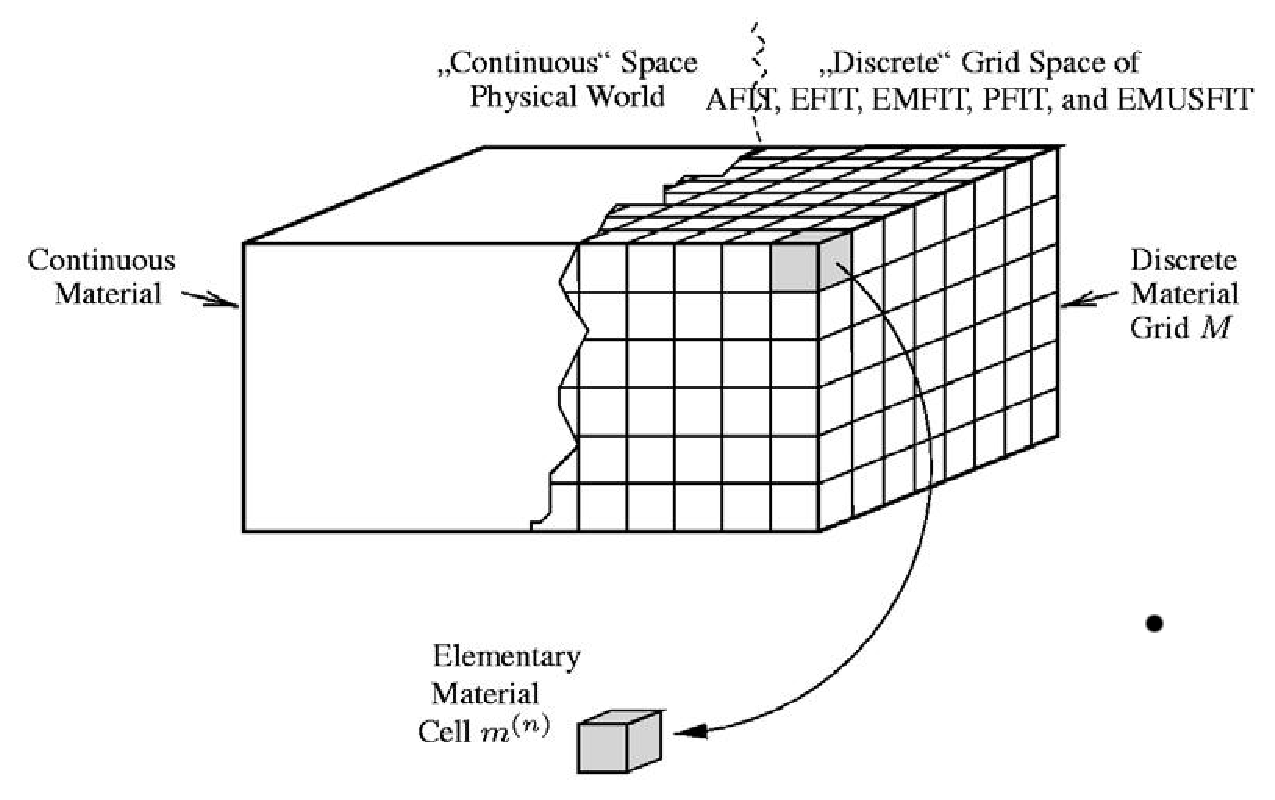
\includegraphics[width=0.8\textwidth]{bilder/discretization_material}
\caption{A discretization of the material in elementary material cells m, defining the material grid M.}
\label{fig:discretization_material}
\end{figure}




                                        % Ein Kapitel des Hauptteils
                                        % Schluss
%Literaturverzeichnis
\begin{spacing}{1.0}                    % Verzeichnisse werden mit einzeiligem Abstand gesetzt
%\bibliographystyle{get_deu_alphadin}							% default styles  get_alphadin} %     
%\bibliographystyle{alpha}
%\bibliographystyle{get_natdin}
%\bibliographystyle{get_eng_natdin}						% f�r englische Texte
\bibliographystyle{unsrtdin}
\bibliography{backmatter/Bibliography}						% Datei 'literatur.bib' wird eingebunden  

\nocite{*}											% include alle Eintr�ge              % Literaturverzeichnis
%\printnomenclature[2cm]
\end{spacing}
%Anh�nge
\appendix
% Anhang
%\chapter{Anhang}
\thispagestyle{empty}
 


\addchap{Appendix}
\section{Power Distribution}
\label{app:powwer_distribution}
%Appendix_power_distribution

This section aims for offering a set of numerical functions to calculating the power distribution along beam propagation in a photonic waveguide. The simplest idea is to compute the power in waveguide and base by integrating power flow density (or Poynting vector $\vec{S}$) at their cross-sections respectively. Meanwhile CST MWS has constructed a cuboid like Fig. \ref{Afig:app_power_distribution01}, which contains all involved objects such as waveguide and TLF, as a total calculation space which is discretized through Finite Integration Technique (FIT) and all variables (see \cite{script_FeldSim} or section \ref{sect:FIT}) from FIT are also available from CST MWS. In following it will be introduced how to calculate the power distribution of a Fiber-to-Chip model (see section \ref{sect:model_simulation}). 
\begin{figure}[ht]
\centering
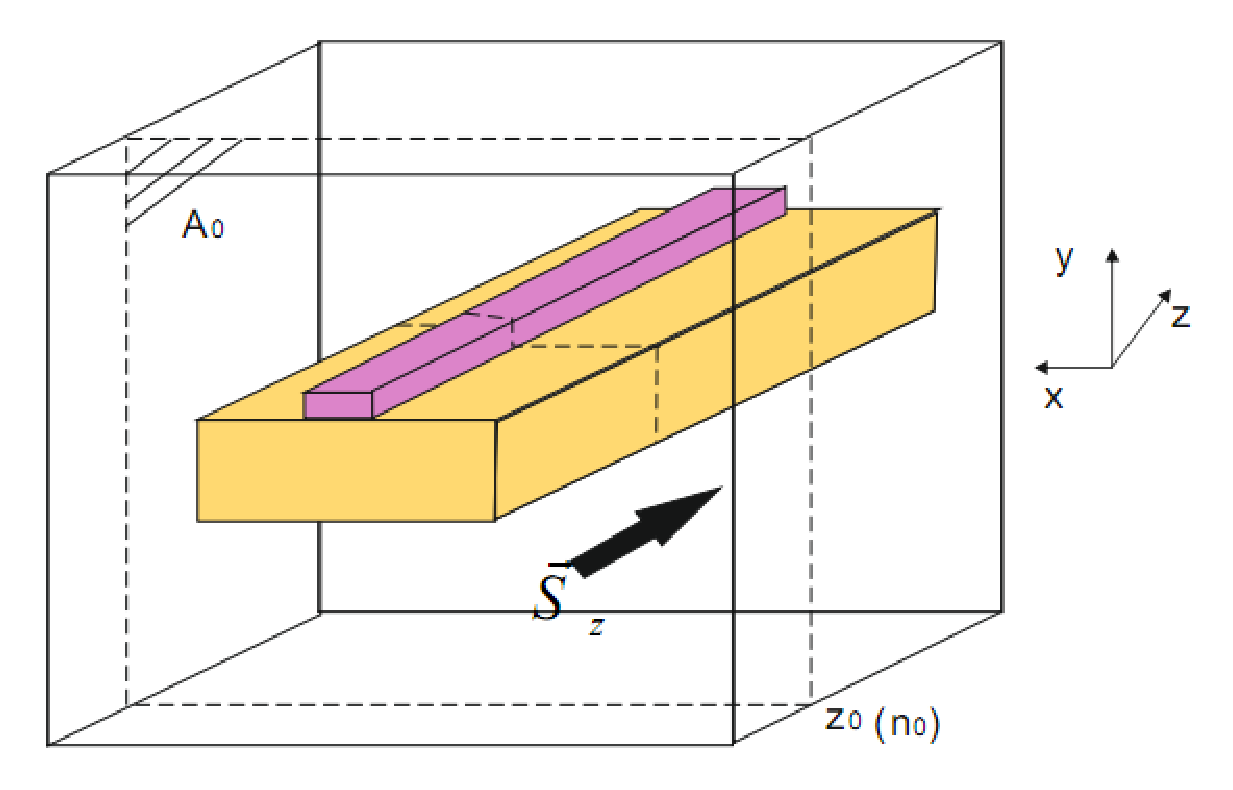
\includegraphics[width=0.7 \textwidth]{bilder/app_power_distribution01}
\caption{Calculation Cuboid in CST.}
\label{Afig:app_power_distribution01}
\end{figure}
The first step is to choose a working plane. Suppose a working plane through point z$_{0}$ at z axis in the total calculation space Fig. \ref{Afig:app_power_distribution01} is given, the point index n$_{0}$ can be determined by its coordinate z$_{0}$. The plane in Fig. \ref{Afig:app_power_distribution02} is divided into small elemental pieces in FIT. The base cross-section is given by four points coordinates (x$_{1}$, y$_{1}$), (x$_{2}$, y$_{2}$), (x$_{3}$, y$_{3}$) and (x$_{4}$, y$_{4}$). Their points indices (n$_{1}$, n$_{2}$, n$_{3}$, n$_{4}$) can also be derived.    
\begin{figure}[ht]
\centering
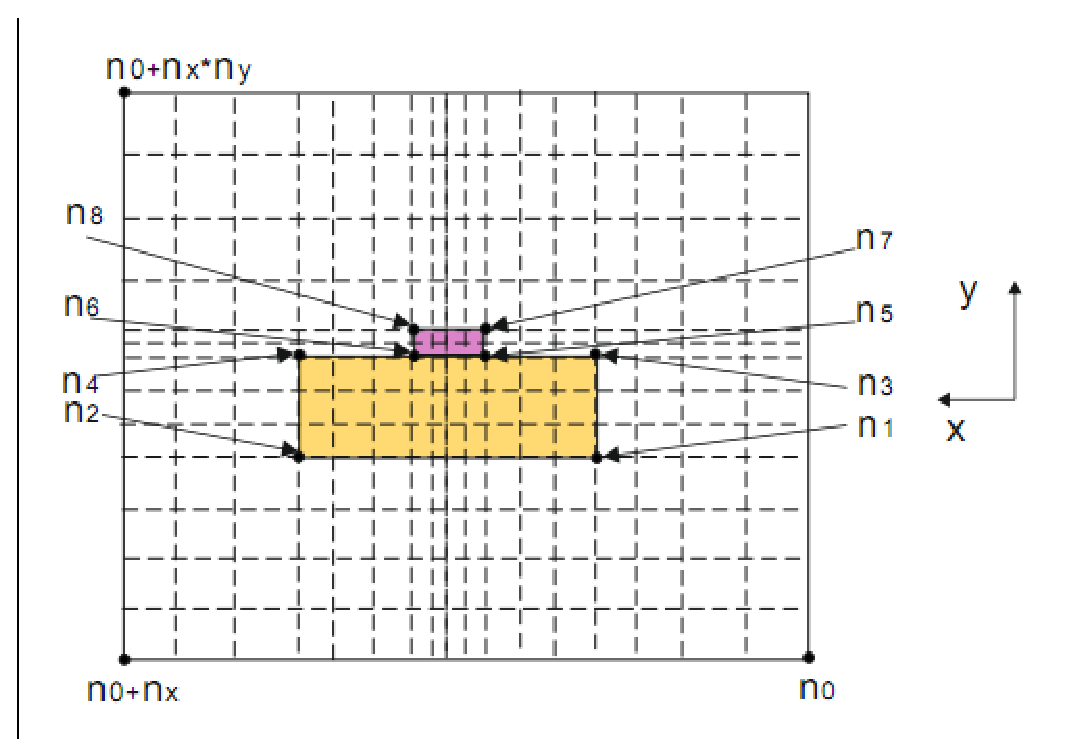
\includegraphics[width=0.7 \textwidth]{bilder/app_power_distribution02}
\caption{Cross-section at z$_{0}$.}
\label{Afig:app_power_distribution02}
\end{figure}
In the next step it is necessary to prepare variables such as elemental 
As is in \cite{script_FeldSim} the complete elemental plane matrix D$_{A}$ is given by (\ref{Aeq:da_matrix}): 
\begin{equation}
D_{A}=Diag\left\{Ax(1),\cdots,Ax(Np),Ay(1),\cdots,Ay(Np), Az(1),\cdots,Az(Np)\right\}
\label{Aeq:da_matrix}
\end{equation}

In the working cross-section only z-components of elemental plane matrix D$_{A}$ are needed:
\begin{equation}
D_{Az}=D_{A}(2*Np+1:3*Np, 2*Np+1:3*Np)
\label{Aeq:daz_matrix}
\end{equation}
Construct a auxiliary matrix $A_{base}$, which composed of only $1$ and $0$ like Fig \ref{Afig:app_Auxiliary_matrix}, to indicate all points indices which are included in base cross-section. 

\begin{equation}
A_{base}=Diag\left\{0,\cdots 0,P_{1},0,\cdots 0, P_{2}, 0,\cdots, P_{m}, 0\cdots\right\}
\label{Aeq:A_matrix}
\end{equation}

\begin{figure}[!ht]
\centering
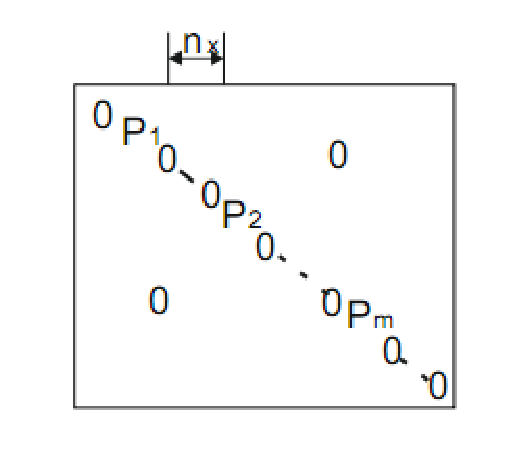
\includegraphics[width=0.5\textwidth]{bilder/app_Auxiliary_matrix}
\caption{Structure of the auxiliary matrix $A$.}
\label{Afig:app_Auxiliary_matrix}
\end{figure}
Where P$_{x}$ are submateix:
\begin{equation}
P_{x}=Diag\left\{1,\cdot,1\right\}_{(n_{2}-n_{1})*(n_{2}-n_{1})}
\end{equation}
And m is given by:
\begin{equation}
m=(n_{3}-n_{1})/n_{x}=(n_{4}-n_{2})/n_{x}
\end{equation}
Then 
\begin{equation}
D_{Abase}=A_{guide}*D_{A}
\end{equation}
Pick z-components of the Poynting vector $S$:
\begin{equation}
S_{z}=S(2*Np+1:3*Np)
\end{equation}
At last the power in base at the plane (for z=z$_{0}$) can be counted up by:
\begin{equation}
P_{base}(z)=\sum(D_{Abase}*S_{z})
\end{equation}

By analogous procedures power in guide cross-section $P_{guide}$ and in total cross-section $P_{total}$ are derived. For observing the power distribution the results are processed by normalization:
\begin{align}
\eta_{guide}&=\frac{P_{guide}}{P_{total}}\\
\eta_{base}&=\frac{P_{base}}{P_{total}}\\
\eta_{air}&=1-\eta_{guide}-\eta_{base}
\end{align}



%% Glossar
\addchap{Glossar}
\thispagestyle{empty}
\label{cha:Glossar} 

Optional kann ein Glossar eingef�gt werden. (optional)
%% Index
Falls gew�nscht kann hier ein Index erstellt werden. (optional)

Dazu m�ssen im Text alle W�rter, die im Index auftauchen sollen mit dem Befehl 
\begin{verbatim}
\index{Befehl}
\end{verbatim}
f�r den Index markiert werden.

Der Index wird dann mit
\begin{verbatim}
\printindex
\end{verbatim}
erstellt werden.

Weitere Informationen bez�glich Indexerstellung sind in der beigef�gten Datei "`/dokumente/makeidx.pdf"' enthalten.

Das fertige Indexverzeichnis sieht dann so aus: (siehe Folgeseite)
\printindex




%% Abk�rzungsverzeichnis
%%\addchap{Abk�rzungsverzeichnis}
\addchap{Abbreviation}
\thispagestyle{empty}
\label{cha:abkurz} 
\textbf{CST MWS} \quad CST Microwave Studio\textregistered\\
\textbf{FIT} \quad Finite Integration Technique\\
\textbf{LAm} \quad longitudinal spherical aberration\\
\textbf{MP} \quad Meridional Plane\\
\textbf{MS} \quad Minimum Spot\\
\textbf{NA} \quad Numerical Aperture\\
\textbf{PP} \quad Paraxial focal Plane\\
\textbf{SMF} \quad Single Mode Fiber\\
\textbf{SPP} \quad Surface Plasmon Polariton\\
\textbf{TLF} \quad Tapered Lensed Fqiber\\




%\cleardoubleemptypage
%\listoftables                           % Tabellenverzeichnis
%(optional)
%\listoffigures                          % Abbildungsverzeichnis
%(optional)

% Die Eidesstattliche Erklaerung auf einer rechten Seite beginnen
\addchap{Erkl�rung}
\thispagestyle{empty}

\vspace*{4cm}

Hiermit versichere ich, dass ich die vorgelegte Diplomarbeit selbst�ndig angefertigt und keine anderen als die angegebenen Quellen und Hilfsmittel verwendet habe.

\bigskip
\bigskip 
\bigskip 
\bigskip 
\bigskip 

\begin{flushright}
\begin{tabular}{c}
%Paderborn, den dd. month yyyy\\
Paderborn, \today\\%dd. month yyyy\\
\bigskip \\
\hrulefill \\
%\dotfill \\
Buyu Xiao\\
\hspace{5cm} \\
\end{tabular}
\end{flushright}
               % Eidesstattliche Erklaerung

\end{document}